\documentclass[12pt]{article}
\usepackage[utf8]{inputenc}
\usepackage[margin=1in]{geometry}
\usepackage[spanish]{babel}\decimalpoint
\usepackage{setspace}\onehalfspacing
\usepackage{parskip} % Espacio entre parrafos.
\usepackage{graphicx} % Para usar comando \includegraphics[]{}
\usepackage{amssymb} % Para usar el simbolo del conj. de los Reales.
\usepackage{amsmath} % Para usar columnas vectoriales.
\usepackage{multirow} % Para unir multiples filas en una tabla.
\usepackage{hyperref} % Siempre debe ser el ultimo paquete.


\setcounter{tocdepth}{2} % Que no incluya subsubsections en la tabla de contenidos (toc).

%================================

\title{Clase 1. Vectores y el Producto Punto.}
\author{MIT 18.02: Multivariable Calculus.}
\date{}


\begin{document}

\maketitle

\begin{abstract}
\noindent En esta primera clase haremos una revisión de conceptos y operaciones básicas con \textbf{vectores}, con un especial énfasis en el \textbf{producto punto} entre dos o más vectores.
\end{abstract}

\section{Vectores.}

Un \textbf{vector} es una \textbf{cantidad} que consiste de una:

\begin{itemize}
\item Dirección.
\item Magnitud (o longitud).
\end{itemize}

\textbf{Toda cantidad que no tenga una dirección}, se califica como \textbf{Escalar} (o cantidad escalar). En general, las palabras ``número'', ``constante'' y ``escalar'' son sinónimos.

Por ejemplo, la magnitud de un vector es un escalar, ya que es solo un número. En cambio, si decimos que ``un vehículo se mueve a $5$ km/hr al norponiente'', aquella cantidad corresponde a un vector.

Un hecho que es bueno tener en cuenta, es que \textbf{dos o más vectores son iguales sí y solo sí sus componentes y dirección son equivalentes}.

%\subsection{Formas de representar a un vector.}

\subsection{Expresando a un vector de forma escrita.}

De forma escrita, los vectores suelen ser representados de dos maneras:
\begin{align*}
  \vec{a} &= \text{vector } a & \mathbf{a} &= \text{vector } a
\end{align*}
En ambos casos nos referimos al vector $a$. En este curso usaremos la notación en negrita.

\subsection{Representación geométrica y componentes de un vector.}

Geométricamente, los vectores se representan como una \textbf{flecha}, donde su largo es la magnitud y el sentido corresponde a la dirección.

%\newpage

\begin{figure}[hbt!]
\centering
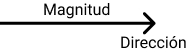
\includegraphics[scale=0.6]{img/vector-arrow.jpg}
\end{figure}

Los vectores son graficados en un \textbf{plano de coordenadas}. Por ejemplo, acá trazamos al vector $\mathbf{a}$ en un plano de tres dimensiones (o un plano $xyz$).

\begin{figure}[hbt!]
\centering
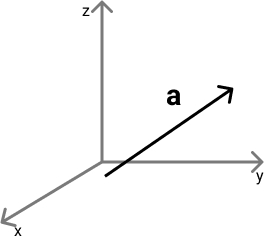
\includegraphics[scale=0.5]{img/vector-xyz-plane.jpg}
\end{figure}

La gráfica de arriba es posible obtenerla cuando conocemos los \textbf{componentes} de un vector, que indican su \textbf{distancia con respecto a sus ejes}. La \textbf{dimensión} de dicho vector está determinado por la cantidad de éstos.

Los componentes de un vector suelen escribirse en paréntesis angulares $\langle \cdot \rangle$. Por ejemplo, si los componentes de un vector $\mathbf{a}$ son $a_{1}$, $a_{2}$ y $a_{3}$, entonces podemos denotarlo como:
\[
  \mathbf{a} = \langle a_{1}, \ a_{2}, \ a_{3} \rangle
\]
donde:
\begin{align*}
  a_{1} &= x_{2} - x_{1} & a_{2} &= y_{2} - y_{1} & a_{3} &= z_{2} - z_{1}
\end{align*}

\subsection{Magnitud de un vector.}

La \textbf{magnitud de un vector} se calcula a partir de sus componentes y se denota como $||\mathbf{a}||$. Sea $\mathbf{a} = \langle a_{1}, \ a_{2}, \ a_{3} \rangle$, su magnitud corresponde a:
\[
  ||\mathbf{a}|| = \sqrt{a_{1}^{2} + a_{2}^{2} + a_{3}^{2}}
\]
Esta fórmula se puede aplicar a vectores de cualquier dimensionalidad y está basada en el \textbf{Teorema de Pitágoras}.

\textbf{Demostración.} Sea $\mathbf{a} = \langle a_{1}, \ a_{2} \rangle$, con $a_{1} = x_{2} - x_{1}$ y $a_{2} = y_{2} - y_{1}$.

Con la distancia horizontal y vertical entre el punto terminal $Q(x_{2}, \ y_{2})$ y el inicial $P(x_{1}, \ y_{1})$ de $\mathbf{a}$, podemos formar un triángulo rectángulo donde el largo de su hipotenusa es $||\mathbf{a}||$.

\begin{figure}[hbt!]
\centering
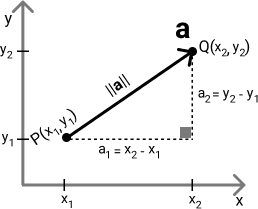
\includegraphics[scale=0.65]{img/magn-proof.jpg}
\end{figure}

Por medio del Teorema de Pitágoras, podemos conocer el valor de $||\mathbf{a}||$ como la raíz cuadrada de la suma de sus catetos $a_{1}$ y $a_{2}$ elevados al cuadrado.
\begin{align*}
  ||\mathbf{a}||^{2} &= (x_{2} - x_1)^{2} + (y_{2} - y_{1})^{2} \\
                     &= a_{1}^{2} + a_{2}^{2} \\
      ||\mathbf{a}|| &= \sqrt{a_{1}^{2} + a_{2}^{2}} \quad \text{(Q.E.D)}
\end{align*}
En ese sentido, si tenemos un vector $\mathbf{a}$ de $n$ componentes, su magnitud se calcula como:
\[
  ||\mathbf{a}|| = \sqrt{a_{1}^{2} + a_{2}^{2} + \cdots + a_{n}^{2}} = \sqrt{\sum_{i = 1}^{n} a_{i}^{2}}
\]

\subsection{Vectores Unitarios.}

Un vector puede ser representado como la suma de las multiplicaciones entre sus componentes y \textbf{vectores unitarios}, que son aquellos magnitud igual a $1$ y se denotan con un $\hat{\cdot}$ arriba.

Por ejemplo, el vector $\mathbf{a} = \langle a_{1}, \ a_{2}, \ a_{3} \rangle$ es equivalente a:
\[
  \mathbf{a} = a_{1}\hat{\mathbf{i}} + a_{2}\hat{\mathbf{j}} + a_{3}\hat{\mathbf{k}}
\]
donde $\hat{\mathbf{i}}$, $\hat{\mathbf{j}}$ y $\hat{\mathbf{k}}$ son \textbf{vectores unitarios} de componentes:
\begin{align*}
  \hat{\mathbf{i}} &= \langle 1, \ 0, \ 0 \rangle &
  \hat{\mathbf{j}} &= \langle 0, \ 1, \ 0 \rangle &
  \hat{\mathbf{k}} &= \langle 0, \ 0, \ 1 \rangle
\end{align*}
y magnitudes:
\begin{align*}
  ||\hat{\mathbf{i}}|| &= \sqrt{1^{2} + 0^{2} + 0^{2}} = 1 &
  ||\hat{\mathbf{j}}|| &= \sqrt{0^{2} + 1^{2} + 0^{2}} = 1 &
  ||\hat{\mathbf{k}}|| &= \sqrt{0^{2} + 0^{2} + 1^{2}} = 1
\end{align*}
Observemos que al sumar estas multiplicaciones, obtenemos el mismo vector escrito con $\langle \cdot \rangle$.
\begin{align*}
\mathbf{a} &= a_{1}\hat{\mathbf{i}} + a_{2}\hat{\mathbf{j}} + a_{3}\hat{\mathbf{k}} \\
           &= a_{1} \langle 1, \ 0, \ 0 \rangle + a_{2} \langle 0, \ 1, \ 0 \rangle + a_{3} \langle 0, \ 0, \ 1 \rangle \\
           &= \langle a_{1}, \ 0, \ 0 \rangle + \langle 0, \ a_{2}, \ 0 \rangle + \langle 0, \ 0, \ a_{3} \rangle \\
\mathbf{a} &= \langle a_{1}, \ a_{2}, \ a_{3} \rangle
\end{align*}
Estas sumas de las multiplicaciones entre una cantidad\footnote{Puede ser un número o un vector. Cuando se aplica a este último se obtiene un nuevo vector.} y una constante, también se conoce como \textbf{Combinación Lineal}.

En general, todo vector de magnitud igual a $1$ es unitario. Por ejemplo, podría interesarnos buscar un \textbf{vector unitario $\hat{\mathbf{i}}$} que esté en la \textbf{misma dirección} de $\mathbf{a}$. Aquello es posible lograrlo de la siguiente forma:
\[
  \hat{\mathbf{i}} = \left(\frac{1}{||\mathbf{a}||}\right) \cdot \mathbf{a}
                   = \left(\frac{1}{||\mathbf{a}||}\right) \cdot \langle a_{1}, \ a_{2}, \ a_{3} \rangle
                   = \left\langle \frac{a_{1}}{||\mathbf{a}||}, \ \frac{a_{2}}{||\mathbf{a}||}, \frac{a_{3}}{||\mathbf{a}||} \right\rangle
\]
La fórmula de arriba se aplica también a aquellos de $n$ dimensiones y se conoce como \textbf{Normalización} del vector $\mathbf{a}$, donde siempre se cumplirá que:
\[
  ||\hat{\mathbf{i}}|| = \sqrt{
                                \left(\frac{a_{1}}{||\mathbf{a}||}\right)^{2} +
                                \left(\frac{a_{2}}{||\mathbf{a}||}\right)^{2} +
                                \left(\frac{a_{3}}{||\mathbf{a}||}\right)^{2}
                              }
                       = 1
\]

\subsection{Vectores y Ángulos.}

Cuando trabajamos con vectores de forma geométrica en un plano, suele ser de interés el ángulo que se forma con respecto a otro objeto.

Por ejemplo, la \textbf{dirección de un vector} de dos dimensiones se puede conocer a partir del ángulo $\theta$ que se forma entre su punto inicial y una recta horizontal que pasa por él. Para ello, podemos ubicarlo en una circunferencia unitaria entre el origen y el punto $(x, \ y)$.

%\newpage

\begin{figure}[hbt!]
\centering
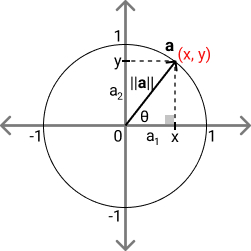
\includegraphics[scale=0.6]{img/direction-vector-1.jpg}
\end{figure}

El radio de una circunferencia es la distancia entre ésta y su centro. En el caso de la unitaria es igual a $1$ y, como vemos en la gráfica de arriba, coincide con la magnitud de $\mathbf{a}$. Por lo tanto, acá $||\mathbf{a}|| = 1$.

También se puede observar que $a_{1} = x - 0$ y $a_{2} = y - 0$, donde $a_{1}$ y $a_{2}$ son las componentes de $\mathbf{a}$ los que, en conjunto, forman un triángulo rectángulo. En ese sentido, con el ángulo $\theta$ podemos usar funciones trigonométricas para conocer su relación con los componentes y la magnitud de este vector:
\begin{align*}
\sin(\theta) &= \frac{a_{2}}{||\mathbf{a}||} = \frac{a_{2}}{1} = a_{2} &
\cos(\theta) &= \frac{a_{1}}{||\mathbf{a}||} = \frac{a_{1}}{1} = a_{1} &
\tan(\theta) &= \frac{a_{2}}{a_{1}} = \frac{\cos(\theta)}{\sin(\theta)}
\end{align*}
Así, con la inversa de una de ellas podemos conocer al ángulo de dirección $\theta$ de un vector.
\begin{align*}
\sin^{-1}(a_{2}) &= \theta &
\cos^{-1}(a_{1}) &= \theta &
\tan^{-1}\left(\frac{a_{2}}{a_{1}}\right) &= \theta
\end{align*}
Por tanto, un vector también puede ser expresado a partir de su ángulo director, puesto que:
\begin{align*}
\sin(\theta) &= \frac{a_{2}}{||\mathbf{a}||} & \cos(\theta) &= \frac{a_{1}}{||\mathbf{a}||} \\
||\mathbf{a}|| \cdot \sin(\theta) &= a_{2} & ||\mathbf{a}|| \cdot \cos(\theta) &= a_{1}
\end{align*}
Y, en consecuencia, $\mathbf{a} = \langle ||\mathbf{a}|| \cos(\theta), \ ||\mathbf{a}|| \sin(\theta) \rangle$ o también $\mathbf{a} = ||\mathbf{a}||\cos(\theta)\hat{\mathbf{i}} + ||\mathbf{a}||\sin(\theta)\hat{\mathbf{j}}$.

Ahora bien, lo anterior solo es aplicable a vectores de dos dimensiones, pero en la siguiente sección veremos una forma obtener el ángulo director con aquellos de tres.

\section{Operaciones entre Vectores.}

\subsection{Adición entre vectores y Multiplicación Escalar.}

En la sección anterior realizamos sumas entre vectores y multiplicaciones escalares. Ahora profundizemos en estas operaciones.

En general, si tenemos dos vectores $\mathbf{a} = \langle a_{1}, \ a_{2}, \ a_{3} \rangle$ y $\mathbf{b} = \langle b_{1}, \ b_{2}, \ b_{3} \rangle$, la \textbf{suma} entre ellos corresponde al siguiente vector:
\[
  \mathbf{a} + \mathbf{b} = \langle a_{1} + b_{1}, \ a_{2} + b_{2}, \ a_{3} + b_{3} \rangle
\]
La suma entre dos vectores se representa geométricamente como el vector que cierra el triángulo que se forma al unir el punto terminal de un vector al inicial del otro (a); o como el vector diagonal del paralelógramo que se forma al juntarlos en sus puntos iniciales (b).

\begin{figure}[hbt!]
\centering
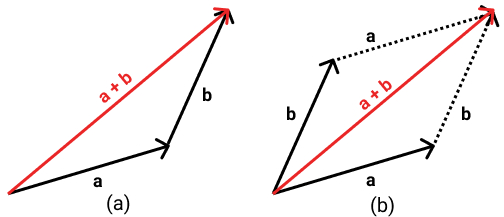
\includegraphics[scale=0.5]{img/vector-sums.jpg}
\end{figure}

En cuanto al producto entre un escalar $c$ y un vector $\mathbf{a} = \langle a_{1}, \ a_{2}, \ a_{3} \rangle$, conocida como \textbf{multiplicación escalar}, es igual al vector:
\[
  c \cdot \mathbf{a} = \langle ca_{1}, \ ca_{2}, ca_{3} \rangle
\]
Cuando a un vector lo multiplicamos por un número o constante, lo que geométricamente estamos haciendo es \textbf{escalarlo}.

\begin{figure}[hbt!]
\centering
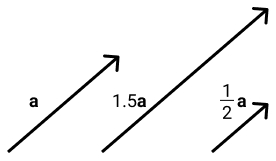
\includegraphics[scale=0.45]{img/scalar-mult.jpg}
\end{figure}

Cuando el escalar $c$ es un \textbf{número negativo} (i.e, $c < 0$), a nivel geométrico significa que \textbf{cambia a su sentido contrario}.

\begin{figure}[hbt!]
\centering
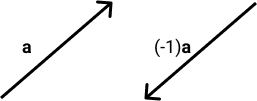
\includegraphics[scale=0.45]{img/scalar-mult-2.jpg}
\end{figure}

Esto también se refleja en la resta $\mathbf{a} - \mathbf{b}$, puesto que en realidad es $\mathbf{a} + (-1)\mathbf{b}$. Es decir, cambia la dirección de $\mathbf{b}$ y, como consecuencia, la magnitud de la suma disminuye.

\begin{figure}[hbt!]
\centering
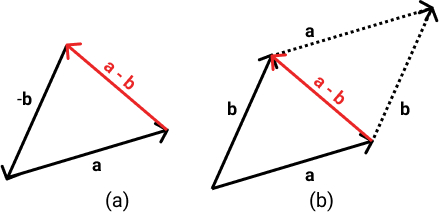
\includegraphics[scale=0.45]{img/vector-subs.jpg}
\end{figure}

Donde:
\[
  \mathbf{a} - \mathbf{b} = \langle a_{1} - b_{1}, \ a_{2} - b_{2}, \ a_{3} - b_{3} \rangle
\]
A continuación tenemos algunas propiedades para la suma de vectores y la multiplicación escalar, donde $\mathbf{0}$ es el \textbf{vector cero}, cuyos componentes y magnitud son iguales a cero.

\begin{table}[hbt!]

\centering

\begin{tabular}{c|c}
Suma de Vectores & Multiplicación Escalar \\
\hline
$\mathbf{a} + \mathbf{b} = \mathbf{b} + \mathbf{a}$ & $c(\mathbf{a} + \mathbf{b}) = c\mathbf{a} + c\mathbf{b}$ \\
$\mathbf{a} + (\mathbf{b} + \mathbf{c}) = (\mathbf{a} + \mathbf{b}) + \mathbf{c}$ & $(c + d)\mathbf{a} = c\mathbf{a} + d\mathbf{a}$ \\
$\mathbf{a} + \mathbf{0} = \mathbf{a}$ & $(cd) \mathbf{a} = c(d\mathbf{a}) = d(c\mathbf{a})$ \\
$\mathbf{a} + (-\mathbf{a}) = \mathbf{0}$ & $1\mathbf{a} = \mathbf{a}$ \\
 & $0\mathbf{a} = \mathbf{0}$ \\
 & $c\mathbf{0} = \mathbf{0}$
\end{tabular}

\end{table}



\subsection{Producto Punto.}

No solo podemos multiplicar a un vector con un escalar, también es posible hacerlo con vectores de igual dimensión. Esta operación recibe el nombre de \textbf{producto punto}\footnote{También conocido como ``producto interno'' o ``producto escalar''.}.

Sean $\mathbf{a} = \langle a_{1}, \ a_{2}, \ a_{3} \rangle$ y $\mathbf{b} = \langle b_{1}, \ b_{2}, \ b_{3} \rangle$, el producto punto entre ellos se calcula como:
\[
  \mathbf{a} \cdot \mathbf{b} = a_{1}b_{1} + a_{2}b_{2} + a_{3}b_{3}
\]
En ese sentido, si $\mathbf{a}$ y $\mathbf{b}$ son de $n$ dimensiones, entonces:
\[
  \mathbf{a} \cdot \mathbf{b} = a_{1}b_{1} + a_{2}b_{2} + \cdots + a_{n}b_{n} = \sum_{i = 1}^{n} a_{i}b_{i}
\]
Algo a tener muy en cuenta, es que \textbf{el producto punto resulta en un valor escalar}. A diferencia de la multiplicacion escalar, que corresponde a un vector.

Con el producto punto también podemos obtener la \textbf{magnitud de un vector}, el cual es igual a la raíz cuadrada del producto punto entre éste y sí mismo. Por ejemplo, sea $\mathbf{a} = \langle a_{1}, \ a_{2} \rangle$, entonces:
\[
  \sqrt{\mathbf{a} \cdot \mathbf{a}} = \sqrt{a_{1}a_{1} + a_{2}a_{2}} = \sqrt{a_{1}^{2} + a_{2}^{2}} = ||\mathbf{a}||
\]
Por lo tanto, si elevamos al cuadrado la magnitud de $\mathbf{a}$, recuperamos el producto punto:
\[
  ||\mathbf{a}||^{2} = \mathbf{a} \cdot \mathbf{a}
\]
A continuación tenemos algunas propiedades del producto punto. Sean $\mathbf{a}$, $\mathbf{b}$ y $\mathbf{d}$ tres vectores de igual dimensiones; y $c$ un escalar:
\begin{align*}
& 1) \ \mathbf{a} \cdot \mathbf{b} = \mathbf{b} \cdot \mathbf{a} \\
& 2) \ (c\mathbf{a}) \cdot \mathbf{b} = c(\mathbf{a} \cdot \mathbf{b}) = \mathbf{b} \cdot (c \mathbf{a}) \\
& 3) \ (\mathbf{a} + \mathbf{b}) \cdot \mathbf{d} = \mathbf{a} \cdot \mathbf{d} + \mathbf{b} \cdot \mathbf{d}
\end{align*}
\textbf{Geométricamente}, el producto punto entre dos vectores $\mathbf{a}$ y $\mathbf{b}$, corresponde a la multiplicación entre sus magnitudes y el coseno del ángulo $\theta$ que se forma entre ellos.
\[
  \mathbf{a} \cdot \mathbf{b} = ||\mathbf{a}|| \cdot ||\mathbf{b}|| \cdot \cos(\theta)
\]
Esto puede ser demostrado usando la \textbf{Ley del Coseno}.

\textbf{Demostración.} Sean $\mathbf{a}$ y $\mathbf{b}$ dos vectores de igual dimensión los que, al ser unidos en sus puntos iniciales, forman entre ellos un ángulo $\theta$.

\begin{figure}[hbt!]
\centering
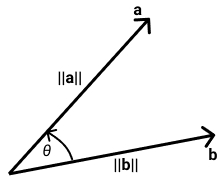
\includegraphics[scale=0.6]{img/dot-product-1.jpg}
\end{figure}

Al trazar al vector $\mathbf{a} - \mathbf{b}$, cuya magnitud es igual a la distancia de los puntos terminales de $\mathbf{a}$ y $\mathbf{b}$, podemos crear un triángulo entre estos tres objetos.

\begin{figure}[hbt!]
\centering
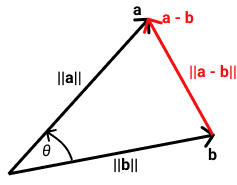
\includegraphics[scale=0.6]{img/dot-product-2.jpg}
\end{figure}

Con $||\mathbf{a}||$, $||\mathbf{b}||$ y $\angle \theta$, podemos conocer a $||\mathbf{a} - \mathbf{b}||$ a partir de la \textbf{Ley del Coseno}, cuya fórmula para este caso es:
\[
  ||\mathbf{a} - \mathbf{b}||^{2} = ||\mathbf{a}||^{2} + ||\mathbf{b}||^{2} - 2 \cdot ||\mathbf{a}|| \cdot ||\mathbf{b}|| \cdot \cos(\theta)
\]
Anteriormente vimos que el producto punto entre un vector y sí mismo es igual a su magnitud al cuadrado. Por lo tanto:
\begin{align*}
(\mathbf{a} - \mathbf{b}) \cdot (\mathbf{a} - \mathbf{b}) &=
    (\mathbf{a} \cdot \mathbf{a}) + (\mathbf{b} \cdot \mathbf{b}) - 2 \cdot ||\mathbf{a}|| \cdot ||\mathbf{b}|| \cdot \cos(\theta) \\
(\mathbf{a} \cdot \mathbf{a}) - (\mathbf{a} \cdot \mathbf{b}) - (\mathbf{b} \cdot \mathbf{a}) + (\mathbf{b} \cdot \mathbf{b}) &=
    (\mathbf{a} \cdot \mathbf{a}) + (\mathbf{b} \cdot \mathbf{b}) - 2 \cdot ||\mathbf{a}|| \cdot ||\mathbf{b}|| \cdot \cos(\theta) \\
-2 \cdot (\mathbf{a} \cdot \mathbf{b}) &= - 2 \cdot ||\mathbf{a}|| \cdot ||\mathbf{b}|| \cdot \cos(\theta) \\
\mathbf{a} \cdot \mathbf{b} &= ||\mathbf{a}|| \cdot ||\mathbf{b}|| \cdot \cos(\theta) \quad (\text{Q.E.D})
\end{align*}
A partir de esta fórmula, podemos conocer a $\theta$ como el arcocoseno (o la función inversa del coseno) del cociente entre el producto punto de $\mathbf{a}$ y $\mathbf{b}$ y la multiplicación de sus magnitudes.
\[
  \theta = \cos^{-1}\left(\frac{\mathbf{a} \cdot \mathbf{b}}{||\mathbf{a}|| \cdot ||\mathbf{b}||}\right)
\]
El ángulo $\theta$ nos entrega información relevante sobre el producto punto entre dos vectores y viceversa también. Esto lo vemos en la siguiente tabla:

\begin{table}[hbt!]

\centering

\begin{tabular}{c|c|c}
$\theta$ en Grados & $\theta$ en Radianes & Prod. Punto \\
\hline
$0^{\text{o}} \leq \theta < 90^{\text{o}}$ & $0 \leq \theta < \pi/2$ & $\mathbf{a} \cdot \mathbf{b} > 0$ \\
$\theta = 90^{\text{o}}$ & $\theta = \pi/2$ & $\mathbf{a} \cdot \mathbf{b} = 0$ \\
$90^{\text{o}} < \theta \leq 180^{\text{o}}$ & $\pi/2 < \theta \leq \pi$ & $\mathbf{a} \cdot \mathbf{b} < 0$
\end{tabular}

\end{table}

Un concepto que veremos mucho al trabajar con vectores, es el de \textbf{ortogonalidad}, que es el sinónimo geométrico de \textbf{perpendicularidad}.

\textbf{Vectores Ortogonales}: Sean $\mathbf{a}$ y $\mathbf{b}$ dos vectores de igual dimensionalidad:
\[
  \mathbf{a} \perp \mathbf{b} \iff \mathbf{a} \cdot \mathbf{b} = 0
\]

\textbf{Ejercicio.} Demuestre por qué la ecuación $x + 2y + 3z = 0$ es un plano.

\textbf{Solución.} Si nos damos cuenta, el lado izquierdo de la ecuación sigue la forma de haber aplicado el producto punto entre dos vectores. Entonces, sean $\mathbf{a} = \langle x, \ y, \ z \rangle$ y $\mathbf{b} = \langle 1, \ 2, \ 3 \rangle$:
\[
  x + 2y + 3z = \mathbf{a} \cdot \mathbf{b} = 0
\]
Como vemos, $\mathbf{a}$ y $\mathbf{b}$ son ortogonales, puesto que el producto punto entre ellos es igual a cero.

El vector $\mathbf{a}$ son las todas las soluciones de la ecuación. Por lo tanto, podemos decir que todas ellas son perpendiculares a $\mathbf{b}$ y la única posibilidad de que así sea, es que la superficie generada sea totalmente plana. Es por ello que concluimos que $x + 2y + 3z = 0$, es un plano.


\subsection{Ángulos Directores de un Vector en Tres Dimensiones.}

Para conocer la dirección de un vector en tres dimensiones, podemos usar la fórmula vista anteriormente para obtener el ángulo entre dos vectores.

En particular, la idea es trabajar el vector expresado en términos de vectores unitarios, porque usaremos los ángulos que se forman entre éstos y el primero.

A continuación tenemos graficado al vector $\mathbf{a} = a_{1}\hat{\mathbf{i}} + a_{2}\hat{\mathbf{j}} + a_{3}\hat{\mathbf{k}}$.

\begin{figure}[hbt!]
\centering
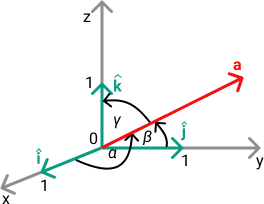
\includegraphics[scale=0.7]{img/dir-angles-3d.jpg}
\end{figure}

Como vemos, entre $\mathbf{a}$ e $\hat{\mathbf{i}}$ está $\angle \alpha$; entre $\mathbf{a}$ y $\hat{\mathbf{j}}$ está $\angle \beta$; y entre $\mathbf{a}$ y $\hat{\mathbf{k}}$ está $\angle \gamma$. Por lo tanto, debido a que en todos ellos podemos aplicar la ley del coseno, estos ángulos los obtenemos como:
\begin{align*}
  \alpha &= \cos^{-1}\left(\frac{\mathbf{a} \cdot \hat{\mathbf{i}}}{||\mathbf{a}|| \cdot ||\hat{\mathbf{i}}||}\right)
          = \cos^{-1}\left(\frac{\mathbf{a} \cdot \hat{\mathbf{i}}}{||\mathbf{a}||}\right) \\
  \beta &= \cos^{-1}\left(\frac{\mathbf{a} \cdot \hat{\mathbf{j}}}{||\mathbf{a}|| \cdot ||\hat{\mathbf{j}}||}\right)
          = \cos^{-1}\left(\frac{\mathbf{a} \cdot \hat{\mathbf{j}}}{||\mathbf{a}||}\right) \\
  \gamma &= \cos^{-1}\left(\frac{\mathbf{a} \cdot \hat{\mathbf{k}}}{||\mathbf{a}|| \cdot ||\hat{\mathbf{k}}||}\right)
          = \cos^{-1}\left(\frac{\mathbf{a} \cdot \hat{\mathbf{k}}}{||\mathbf{a}||}\right)
\end{align*}



\end{document}
